\chapter{Introduction}


\epigraph{[Quantum computation] does not merely make computer science
a branch of physics. \\ It also makes part of experimental physics into a branch of computer science}{\textit{Quantum theory, the Church-Turing principle \\ and the universal
quantum computer \\ -- David Deutsch}}

Quantum mechanics is one of the most well-tested theories in existence [REF?]. It is also one of the most unintuitive, revealing aspects of nature at nanoscopic scales which are entirely incompatible of our own experience of the world. \\

Quantum mechanics has two key facets. The first, from which the field derives its moniker, is the quantisation of properties such as charge, angular momentum, and energy. This property has already changed the world substantially over the course of the last 70 years. Among technologies such as the laser and magnetic resonant imaging (MRI), perhaps the greatest impact has been made through the manipulation of semiconductor technology. Since the invention of the first transistor in 1947 \cite{Bardeen1948}, this semiconductor technology has laid the groundwork for scalable computers, bringing us into the information age. \\

The development of this technology comes at a critical time in the conventional silicon industry. The famous Moore's law, hypothesised in its current form in 1975, stated that the number of transistors per square inch would double every two years. This law models the exponential scaling of computing power since its conception incredibly well, as we can see in \autoref{fig:Moore's_Law}. This was driven partly by the cost and power consumption per transistor going down as feature sizes decreased \cite{MooresLawEconomist}.  However, now increasingly small feature sizes have resulted in energy efficiencies and profitability are starting to plateau, while technical issues continue to increase. These issues are in part due to quantum effects such as tunnelling.  \\


\begin{figure}[h!]
	\centering
	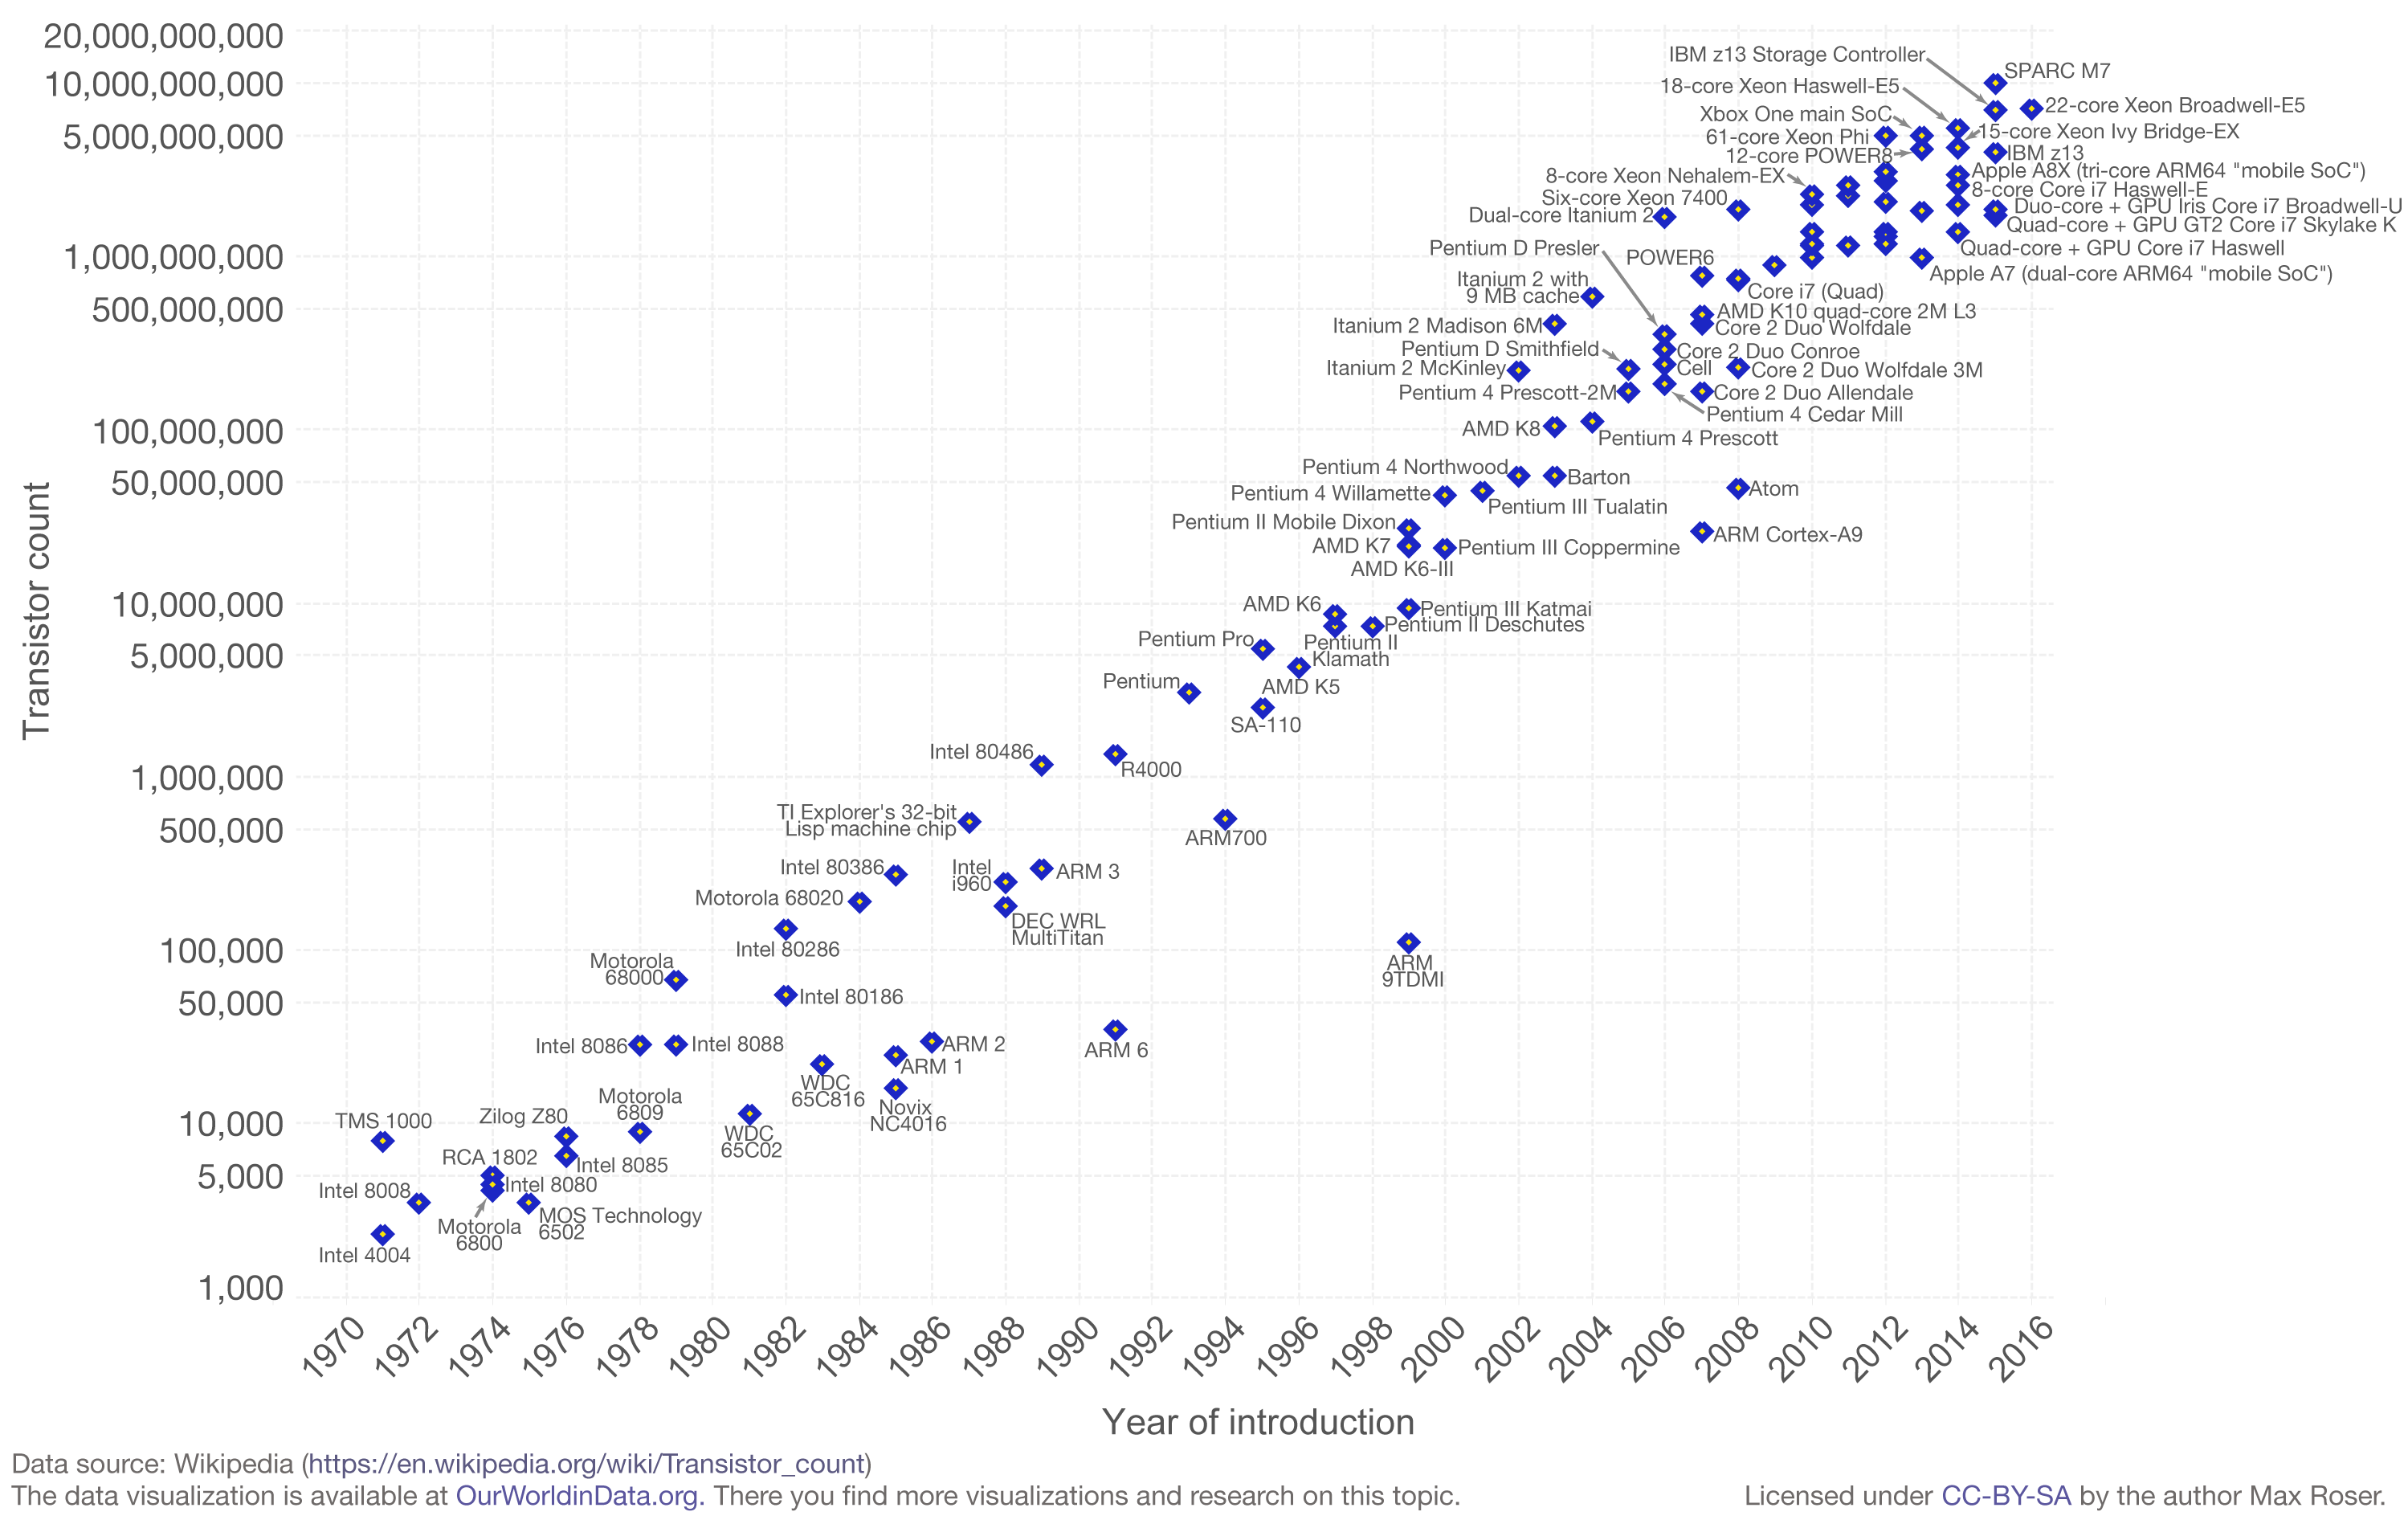
\includegraphics[width = \linewidth]{Moores_Law.png}
	\caption{Chart showing Moore's law, with a logarithmic increase in transistor 	count on each chip from 1970-2016.}
	\label{fig:Moore's_Law}
\end{figure}

This example of tunnelling is related to the so-called `wave-particle duality' which is the second key feature of quantum mechanics. Which is causing these issues may the solution in addition to the problem. The distinction between waves and particles, whose behaviour is well established in classical physics, becomes blurred. \textbf{Every object in the universe, if the correct energy and length scales are chosen, will display both of these aspects to some degree.} \\

It is in this property in which lies the tantalising promise of quantum computing. Particles like electrons, which have comprised the backbone of electricity and classical information for the past century, have the ability to behave in a wave-like manner: they could contain not just the binary bit choices of 0 or 1,  but one of an infinite number of continuous values, called `qubits'. Combined with entanglement to allow our qubits to influence each other while in this state, we can harness a sort of parallelism that results from the wave-like nature of controlled particles.  \\


While in general it is doubtful that a quantum computer will be generically  `faster' than a classical computer, and it is much harder to engineer, we do have significant potential to outperform conventional computers at certain tasks. While the amount of information processing in a conventional computer scales linearly with the number of bits, a quantum computer scales exponentially with the number of qubits for these tasks. Thus adding a single extra qubit could double the computing power. These are discussed, along with the quantum algorithms used to implement them, in Chapter \autoref{Algorithms and applications}. At the point when quantum computers are able to outperform classical supercomputers at a task, the so-called `quantum supremacy' will have been achieved. \\

These tasks range from \ldots\\ 

 

However, achieving this potential does not come without significant difficulty. Readout or detection of the information in the qubit destroys the information contained within, resulting in us reverting to the classical bit values with some probability. Furthermore, the technology is still very young and undeveloped. Algorithms exist for many of the applications above, but there may be many more as yet undiscovered. Academic institutions , large corporations (including Google \cite{bristlecone}, IBM, Intel) and small start-ups (Rigetti, \cite{rigettihome}) alike have invested heavily in hardware. There are a wide range of platforms and architectures, including but not limited to superconducting qubits \cite{bristlecone}, ion traps [REF], quantum dots [REF], spin qubits in silicon [REF], and silicon photonics [REF]. \\


One crucial area that remains comparatively underdeveloped is software. It will be crucial to provide this missing link between the theoretical algorithm and its implementation on a quantum computer. Ideally `quantum' programming should adopt many of the features as its classical counterpart: it should be usable by any person without understanding the details of the hardware being used, it 


Over the next few years and decades quantum computing is likely to become a reality. It will be crucial when this becomes the case that people are able to understand how to use these machines in order to harness their applicability to the areas of mathematics, computer science, chemistry and finance. This guide is designed to be an introduction to the science of quantum computers and the current state of the field. Initially we explain in more depth how quantum computers work and their differences to classical computers in Chapter \autoref{TheBasics}. Since in the short-term, quantum computers are likely to be noisy, error-prone and limited in scale, we discuss how they can be used in this regime in \autoref{Short term quantum computing}. \\

Once the engineering of quantum computers have been improved, then a host of more impressive applications can be demonstrated, which are considered in chapter \autoref{Algorithms and applications}. We examine the programming languages that will be able to interface between the algorithms and the quantum computer in chapter \autoref{Programming a future universal quantum computer}, and hardware-specific implementations and architectures in chapter \autoref{Implementations}. \\

A more complete description of quantum mechanics is given in chapter \autoref{Advanced Topics} for any interested party. 
